\documentclass[letterpaper,12pt]{article}

\setlength{\topmargin}{0in}
\setlength{\textheight}{9.0in}
\setlength{\textwidth}{6.5in}
\setlength{\columnsep}{0.25in}
\setlength{\headheight}{0in}
\setlength{\headsep}{0in}
\setlength{\oddsidemargin}{0.0in}
\setlength{\evensidemargin}{0.0in}
\setlength{\topskip}{0in}
\usepackage{times}
\usepackage{mdwlist}
\usepackage{hyperref}
\usepackage{array}
\usepackage{multicol}
\usepackage{enumitem}
\usepackage{graphicx}
\usepackage{amsmath}
\hypersetup{colorlinks=true}
\renewcommand{\baselinestretch}{1.00}

\newcounter{exanum}
\setcounter{exanum}{1}
\newcommand{\exercise}{\subsubsection*{Exercise \#\theexanum: \refstepcounter{exanum}}}

\newcommand{\duedate}{end of day, October 03, 2019}

\newcommand{\courseyear}{Fall 2019}
\newcommand{\system}{Stampede2}

\input{vc}


\begin{document}
\begin{flushright}
\VCDateISO \\
Rev: \VCRevision
\end{flushright}

\vspace*{0.05cm}
\subsection*{Tools and Techniques for Computational Science - \courseyear{}}
\vspace*{-.2cm}
\noindent{{\large \em Assignment \#2}

\vspace*{15pt}

\noindent {\bf Setup}: Before starting this homework, enable your personal
git repository for the class by going to the following URL: 
\href{https://classroom.github.com/a/8thETCJZ}{https://classroom.github.com/a/8thETCJZ}. 
Your repository will be created dynamically and will be empty to start.

\subsection*{Shell Scripts, Batch Jobs}

Please answer the following questions and commit your resulting
scripts to your assigned GitHub repository
(https://github.com/uthpc/student-{\em yourgithubId}.git).  You should
commit periodically while working on the shell scripts and have a
minimum of 5 commits per script (with relevant commit
messages). Please store the results in a \texttt{hw02/} subdirectory
of your repository and name the files as requested in each
exercise. This homework is due by \duedate. \\

\noindent{\bf Please tag your repository with a name of ``hw02'' after
  you have completed the assignment and pushed all requested files to
  your repo} (and please, don't forget to push from your local repo).
\begin{verbatim}
(master)$ git tag -a "hw02" -m "tagging completion of hw02"
(master)$ git push --tags
\end{verbatim}

\noindent {\em Note}: scripts requiring command-line arguments to run should print the
script's intended usage and exit with an error if the minimum number
of arguments is not provided.

\noindent\rule{\textwidth}{0.4pt} \\

\exercise

(10 pts) Write a shell script (in Bash) named \texttt{add.sh} 
that will add two integers supplied as command line arguments. 

\vspace*{20pt}

\exercise 

(15 pts) Write a shell script (in Bash) named \texttt{factorial.sh} that uses a
while loop and \texttt{expr} to calculate the factorial of a supplied
number. 

\clearpage
\exercise

(15 pts) Write a shell script (in Bash) named \texttt{tri.sh} that uses a for loop to generate
the following output:

\begin{verbatim}
      1
     2 2
    3 3 3
   4 4 4 4
  5 5 5 5 5
      .
     . .
    . . .
   . . . .
  . . . . .

\end{verbatim}


\exercise

{\bf Part I} (20 pts): Write a shell script (in Bash) named \texttt{pi.sh} to
estimate the value of $\pi$ using a Monte Carlo method. To do this, consider a
circle of radius=1 enclosed by a 2x2 square as shown in
Figure~\ref{fig:circle}.  If we draw random samples for (x,y) coordinates in
the upper right-hand quadrant from the range (0,0) to (1,1), each point can be
classified as being within the circle ($N_i$, the green points), or outside the
circle ($N_o$, the red points). The ratio of the area of the quarter circle to the area
of the quarter square is: $\frac{1}{4}\pi r^2 / \frac{1}{4}(4r^2) = \pi / 4$. Using Monte Carlo sampling and
counting how many points fall within the circle, we can approximate the same
area ratio as $\pi / 4 \approx N_i / N_{samples}$. Consequently, we can
estimate the value of $\pi$ via:

\begin{equation*}
\pi \approx \frac{4 \, N_i}{N_{samples}}
\end{equation*}

\begin{figure}[h]
\begin{center}
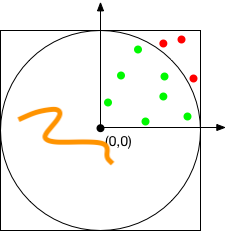
\includegraphics[width=2.2in]{pi-circle.png}
\end{center}
\vspace*{-.7cm}
\caption{Circle of radius 0.5 enclosed by a 1x1 square. 
}
\label{fig:circle}
\end{figure}

To implement this exercise, you will need a random number generator
that can be used to draw samples to generate floating-point coordinates
in the range (0,1).  There are multiple ways to do this: one simple
way is to leverage the built-in random integer generator in Bash
available via the \texttt{\$RANDOM} environment variable (consult man
page of \texttt{bash} for more details). Since this built-in feature
supplies integer samples in the range 0 to 32767, you need to augment
the result to obtain a floating-point number in the desired range. An
example one-liner for doing this using our friendly \texttt{bc}
calculator is as follows:

\begin{verbatim}
echo "scale=15; $RANDOM/32767" | bc -l
\end{verbatim}

Use the above, or another approach in your shell script to define a
Bash function named \texttt{RandomDraw} to generate a random sample in
your script. This function should be called from within the sampling
loop. Your script should take a single integer as input defining the
total number of samples to perform ($N_{samples}$). To evaluate the
quality of the estimate, your script should compute the relative error
as $e_{rel} = |\pi_{est} - \pi|/\pi$. Upon completion, your script
should output a single line to stdout with the following information:

\begin{verbatim}
N_samples N_i N_o pi_estimate e_rel
\end{verbatim}

%\clearpage
\noindent{\bf Runs}: Create a single SLURM job script for use on
Stampede2 to run your \texttt{pi.sh} script sequentially for
$N_{samples}$ = 10, 100, 500, 1,000, 5,000, 10,000, and 50,000.  Save
the results to a file named \texttt{pi.script.log} and append the time
(in seconds) required to complete each run as the 6th column entry in
the file. Note: you can either add this timing incrementally, or save
the timings to a temporary file and join appropriately. The
\texttt{/bin/time} command we highlighted in class has an option to
send the resulting timing to a file (and can also append to a file)
which you may find convenient in your job script. \\

\noindent Commit the job script and results file from a job on Stampede2 to your
GitHub repo. 

\noindent\rule{2cm}{0.4pt}  \\

\noindent {\bf Part II} (20 pts): Repeat the exercise from Part I
implementing the same Monte Carlo method to estimate~$\pi$ using a
compiled language (C/C++ or Fortran). Note: if you use the
\texttt{rand()} function from the standard C library as the source of
the random number generator, the seed value is the same upon each
execution unless you specify otherwise. A common practice is to use a
seed based on the current time which can be accomplished as
follows in C:

\begin{verbatim}
#include<stdlib.h>
#include<time.h> 

srand(time(0));
\end{verbatim}

\noindent{\bf Runs}: Create a second SLURM job script for use on
Stampede2 to run your compiled $\pi$ estimator for the same sample
counts used in Part I. Save the results to a file named
\texttt{pi.compiled.log} and commit the src code, job script, and
results file from a job on Stampede2 to your repo. 

\clearpage
\noindent\rule{2cm}{0.4pt} \\

\noindent {\bf Part III} (20 pts): Using the compiled binary created
for Part II and the parametric job launcher demo'd in class, create a
third SLURM job script and any necessary files/scripts to run your
binary (in parallel) until a certain level of precision is obtained
for the $\pi$ estimate.  Recall that we can use the job launcher as a
convenience mechanism to aggregate multiple independent jobs by
specifying individual tasks to perform in a text file. The general
approach is as follows:

\begin{itemize}

\item Configure your job script to request 1 Skylake node and 48 cores
\item For efficiency, design your job to perform samples in chunks and
  continue iterating until the desired level of precision is
  obtained. Let the chunk size be 
  $N_{chunk} = 960,000,000$ samples (note that this value is evenly divisible by 48).
\item At each iteration, run your binary in parallel to complete the
  $N_{chunk}$ samples. Once completed, use the aggregate results to
  compute the current estimated value for $\pi$ (using results from
  current and all previous iterations). If the value is not within the
  desired tolerance, execute another iteration. Repeat until the
  desired tolerance is achieved.
\item Since we expect each run of your executable to take roughly the
  same amount of time, use a simple scheduler with the parametric job
  launcher by including the following in
  your job script:
 \texttt{export LAUNCHER\_SCHED=interleaved}

\item Stopping criteria: the desired tolerance to achieve is: $e_{rel} < 5.0 x 10^{-6}$

\item At each iteration, append the current iteration, $N_{samples}$,
  $\pi_{est}$, $e_{rel}$, and the accumulated runtime (in secs) to a
  file named \texttt{iter.log}. Example file format will be shown below.

\end{itemize}

\noindent{\bf Runs}: Run your parametric job on Stampede2 and commit
the job script, launcher related files, \texttt{iter.log}, and the
SLURM job output to your repo. The \texttt{iter.log} file should have a
comment in the first line highlighting the order of the variables. An
overview of the expected file format is shown below. Note that spacing
between values is not important, just make sure to have at least 1
space between values.

\begin{verbatim}
# iter num_samples num_i pi relative_error time_accum
1 960000000 xxx  xxx xxx  xx
2 1920000000 xxx xxx xxx  xx
.
.
.
\end{verbatim}

\end{document}
